\section{Sensitivity to Key Hyperparameters}
\label{sec:ch6_ablation}

The preceding sections evaluated the final AttackDRO++ configuration under
whitebox, class-wise, and graybox settings. Those results show how the method
behaves once the design choices are fixed, but they do not explain how sensitive
the method is to those choices. This section therefore studies three practical
hyperparameters: the number of discovered clusters, the strength of the uniform
anchor, and the frequency with which clusters are refreshed.

These ablations are intended as configuration guidance rather than as a second
main comparison. Unless otherwise stated, they use the same CIFAR-10, ResNet-18,
source-attack, and evaluation-attack protocol defined in Chapter~\ref{chap:experimental_setup}.
Mean(8) and Worst(8) follow the definitions in Section~\ref{sec:ch5_evaluation_metrics}:
both are computed over the eight non-AutoAttack evaluation attacks, while
AutoAttack-$\ell_\infty$ is reported separately.

\subsection{Number of Clusters: How Many Groups Are Needed?}
\label{subsec:ch6_ablation_num_clusters}

The number of clusters controls the granularity of the latent groups used by
AttackDRO++. If $K$ is too small, distinct failure modes may be merged into the
same group, making the Cluster-DRO correction too coarse. If $K$ is too large,
the minibatch may be split into many small groups, making group-loss estimates
noisier and the cluster weights less stable.

Because $K$ controls the trade-off between coarse grouping and noisy small groups,
Table~\ref{tab:ch6_ablation_num_clusters} tests whether AttackDRO++ is sensitive to
cluster granularity. Across the available runs, all settings remain close in Mean(8), with differences
well below one percentage point. The default $K=4$ setting gives the highest
Worst(8) among the tested settings and remains competitive in Mean(8), while
$K=2$ is slightly more coarse and $K=6$ or $K=10$ do not provide a clear gain.
The $K=10$ setting uses only two valid runs and should be interpreted
as weaker evidence than the other cluster-count settings.

\begin{table}[H]
\centering
\caption{Number-of-clusters ablation for AttackDRO++ with anchor strength
$\lambda_{\mathrm{DRO}}=0.35$. Values are robust accuracy (\%) reported as
mean $\pm$ standard deviation across available runs. Mean(8) and Worst(8) are
computed over the eight non-AutoAttack attacks; AutoAttack-$\ell_\infty$ is
reported separately. Bold values indicate the best setting for each metric.}
\label{tab:ch6_ablation_num_clusters}
\small
\setlength{\tabcolsep}{4pt}
\renewcommand{\arraystretch}{1.08}
\begin{tabular}{lccccc}
\toprule
Setting & $K$ & Runs & Mean(8) $\uparrow$ & Worst(8) $\uparrow$ & AutoAttack $\uparrow$ \\
\midrule
Coarse grouping
& 2 & 3
& $62.33 \pm 0.06$
& $45.13 \pm 0.27$
& $40.95 \pm 0.90$ \\

Default grouping
& 4 & 3
& \bestval{62.35 $\pm$ 0.20}
& \bestval{45.33 $\pm$ 0.25}
& \bestval{41.14 $\pm$ 1.15} \\

Finer grouping
& 6 & 3
& $62.28 \pm 0.14$
& $45.17 \pm 0.47$
& $40.95 \pm 1.30$ \\

Very fine grouping
& 10 & 2
& $62.35 \pm 0.09$
& $45.17 \pm 0.08$
& $40.62 \pm 1.11$ \\
\bottomrule
\end{tabular}
\end{table}

\begin{figure}[H]
    \centering
    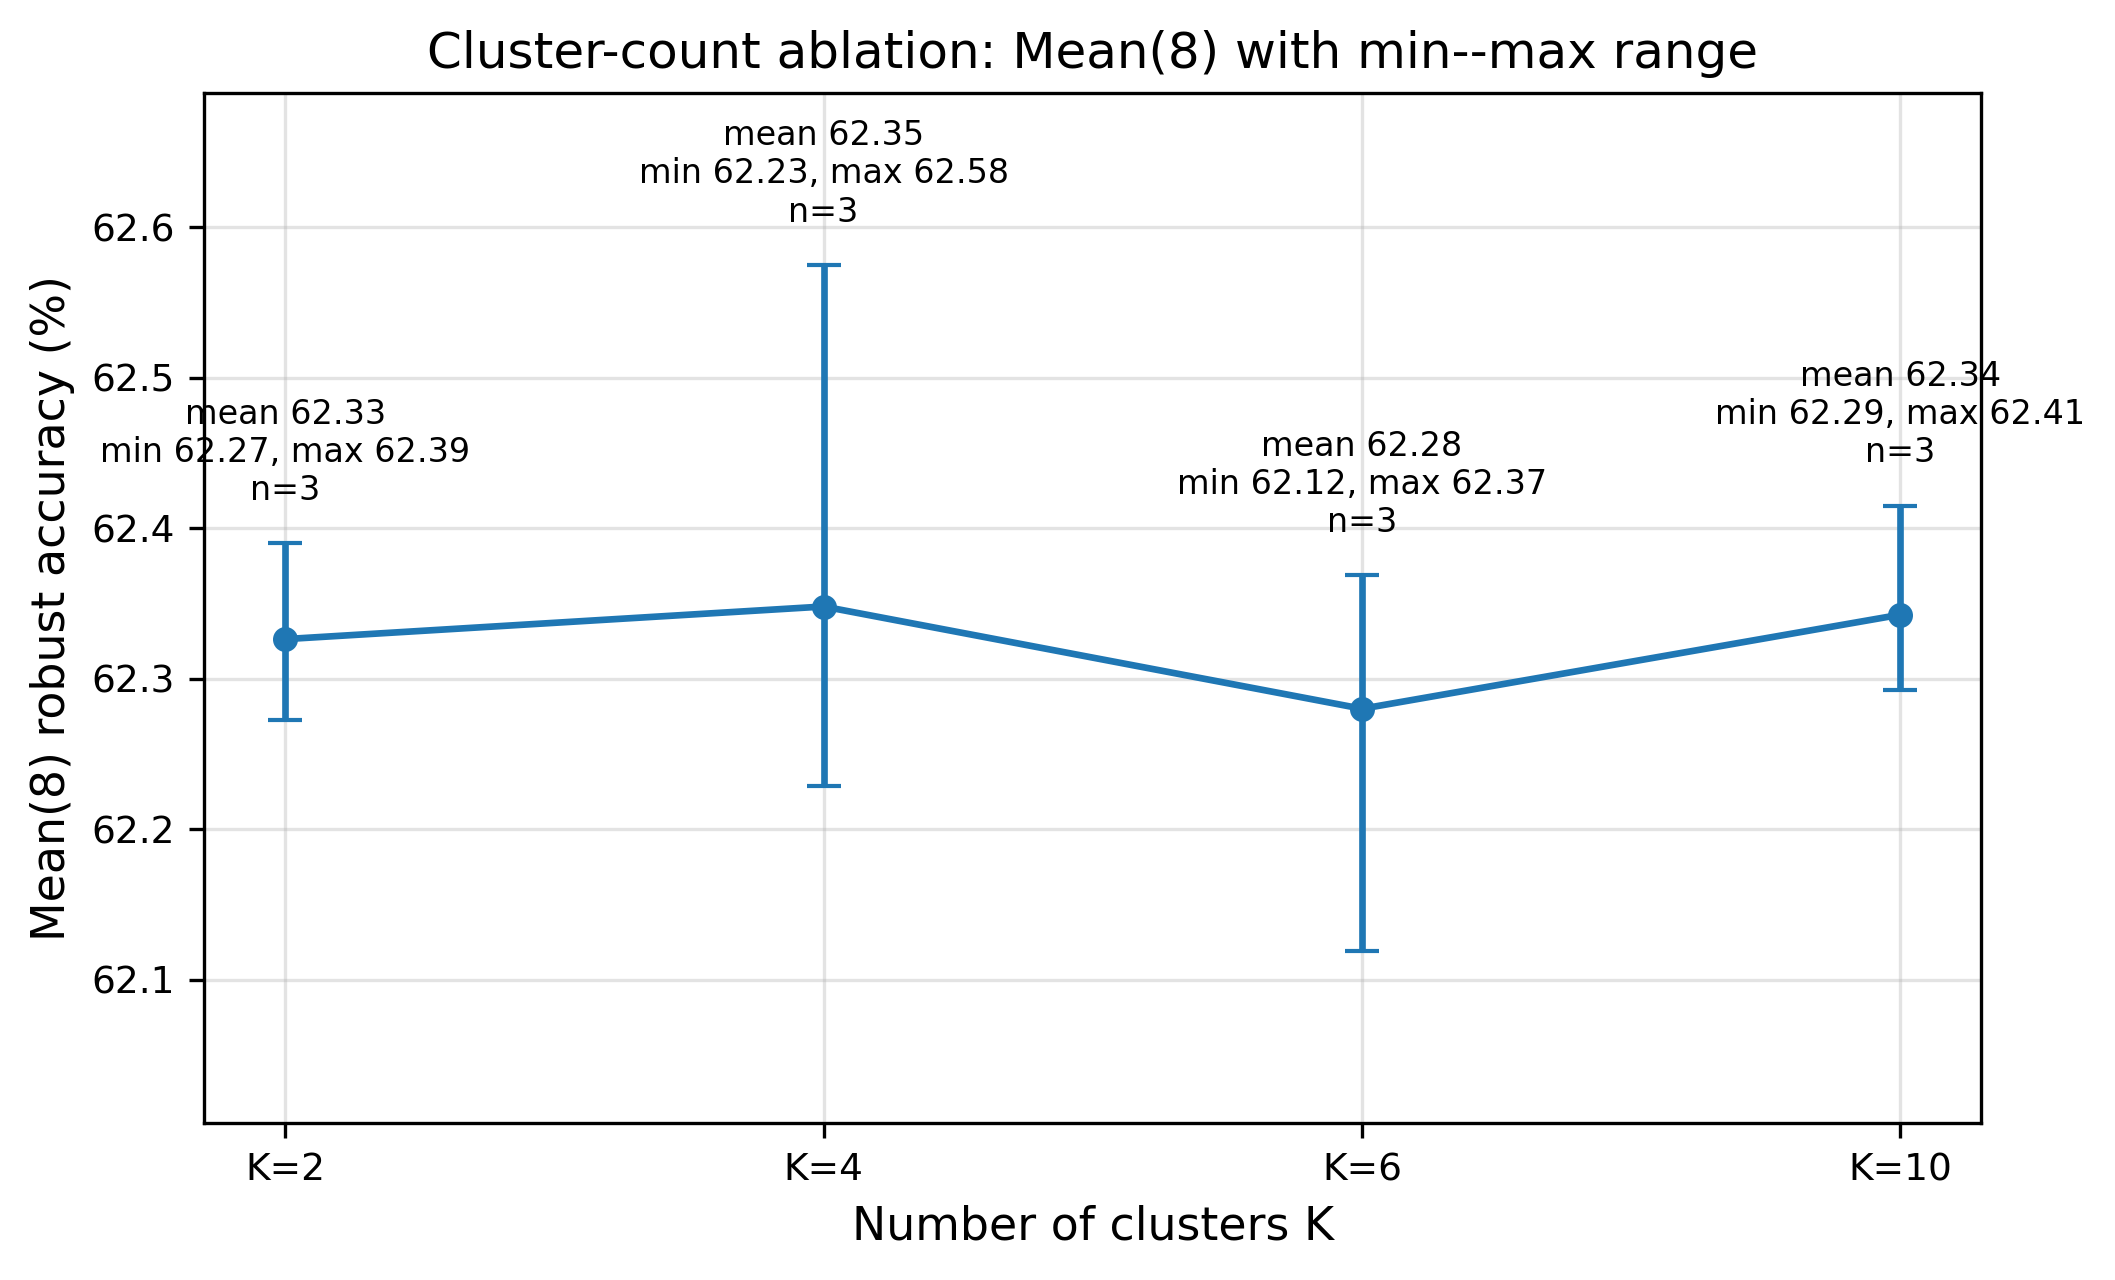
\includegraphics[width=0.82\linewidth]{figures/ablations/ablation_num_clusters.png}
    \caption{Sensitivity of AttackDRO++ to the number of clusters. Points show Mean(8) robust accuracy with the min-to-max range across available runs; Mean(8) is computed over the eight non-AutoAttack evaluation attacks.}
    \label{fig:ch6_ablation_num_clusters}
\end{figure}

The ablation supports using a moderate number of clusters rather than treating
the cluster count as a highly tuned parameter. The default $K=4$ is expressive
enough to go beyond the two source attack identities, but it does not fragment
the training batch as aggressively as larger values. Therefore, the evidence
supports $K=4$ as a stable practical choice, not as a universally optimal cluster
count.

\subsection{Anchor Strength: Finding a Stable Trade-off}
\label{subsec:ch6_ablation_anchor_strength}

The anchor strength $\lambda_{\mathrm{DRO}}$ controls the interpolation between
the uniform multi-attack ERM objective and the adaptive Cluster-DRO objective.
A smaller value keeps training closer to the uniform baseline, while a larger
value gives the cluster-reweighted loss more influence. In this ablation, the
previous $\lambda_{\mathrm{DRO}}=1.0$ setting is removed because it corresponds
to an overly aggressive Cluster-DRO setting and is not part of the final
candidate set.

Because the anchor controls how far the objective can move away from uniform Multi-AT,
Table~\ref{tab:ch6_ablation_anchor_strength} tests three practical anchor strengths.
The differences are again small, but the moderate setting
$\lambda_{\mathrm{DRO}}=0.35$ gives the strongest Mean(8), Worst(8), and
AutoAttack values among the tested settings. The lower value
$\lambda_{\mathrm{DRO}}=0.20$ remains close, suggesting that the method does not
require a sharply tuned anchor. The higher value $\lambda_{\mathrm{DRO}}=0.50$
slightly reduces Mean(8) and AutoAttack, which is consistent with the idea that
too much emphasis on adaptive cluster weighting can reduce the stabilizing effect
of the uniform multi-attack baseline.

\begin{table}[H]
\centering
\caption{Anchor-strength ablation for AttackDRO++ with $K=4$. Values are robust
accuracy (\%) reported as mean $\pm$ standard deviation across three runs.
Mean(8) and Worst(8) are computed over the eight non-AutoAttack attacks;
AutoAttack-$\ell_\infty$ is reported separately. Bold values indicate the best setting for each metric.}
\label{tab:ch6_ablation_anchor_strength}
\small
\setlength{\tabcolsep}{4pt}
\renewcommand{\arraystretch}{1.08}
\begin{tabular}{lcccc}
\toprule
Anchor strength $\lambda_{\mathrm{DRO}}$ & Runs & Mean(8) $\uparrow$ & Worst(8) $\uparrow$ & AutoAttack $\uparrow$ \\
\midrule
$0.20$
& 3
& $62.28 \pm 0.09$
& $45.01 \pm 0.40$
& $41.08 \pm 1.66$ \\

$0.35$ (default)
& 3
& \bestval{62.35 $\pm$ 0.20}
& \bestval{45.33 $\pm$ 0.25}
& \bestval{41.14 $\pm$ 1.15} \\

$0.50$
& 3
& $62.24 \pm 0.18$
& $45.24 \pm 0.40$
& $40.24 \pm 1.09$ \\
\bottomrule
\end{tabular}
\end{table}

\begin{figure}[H]
    \centering
    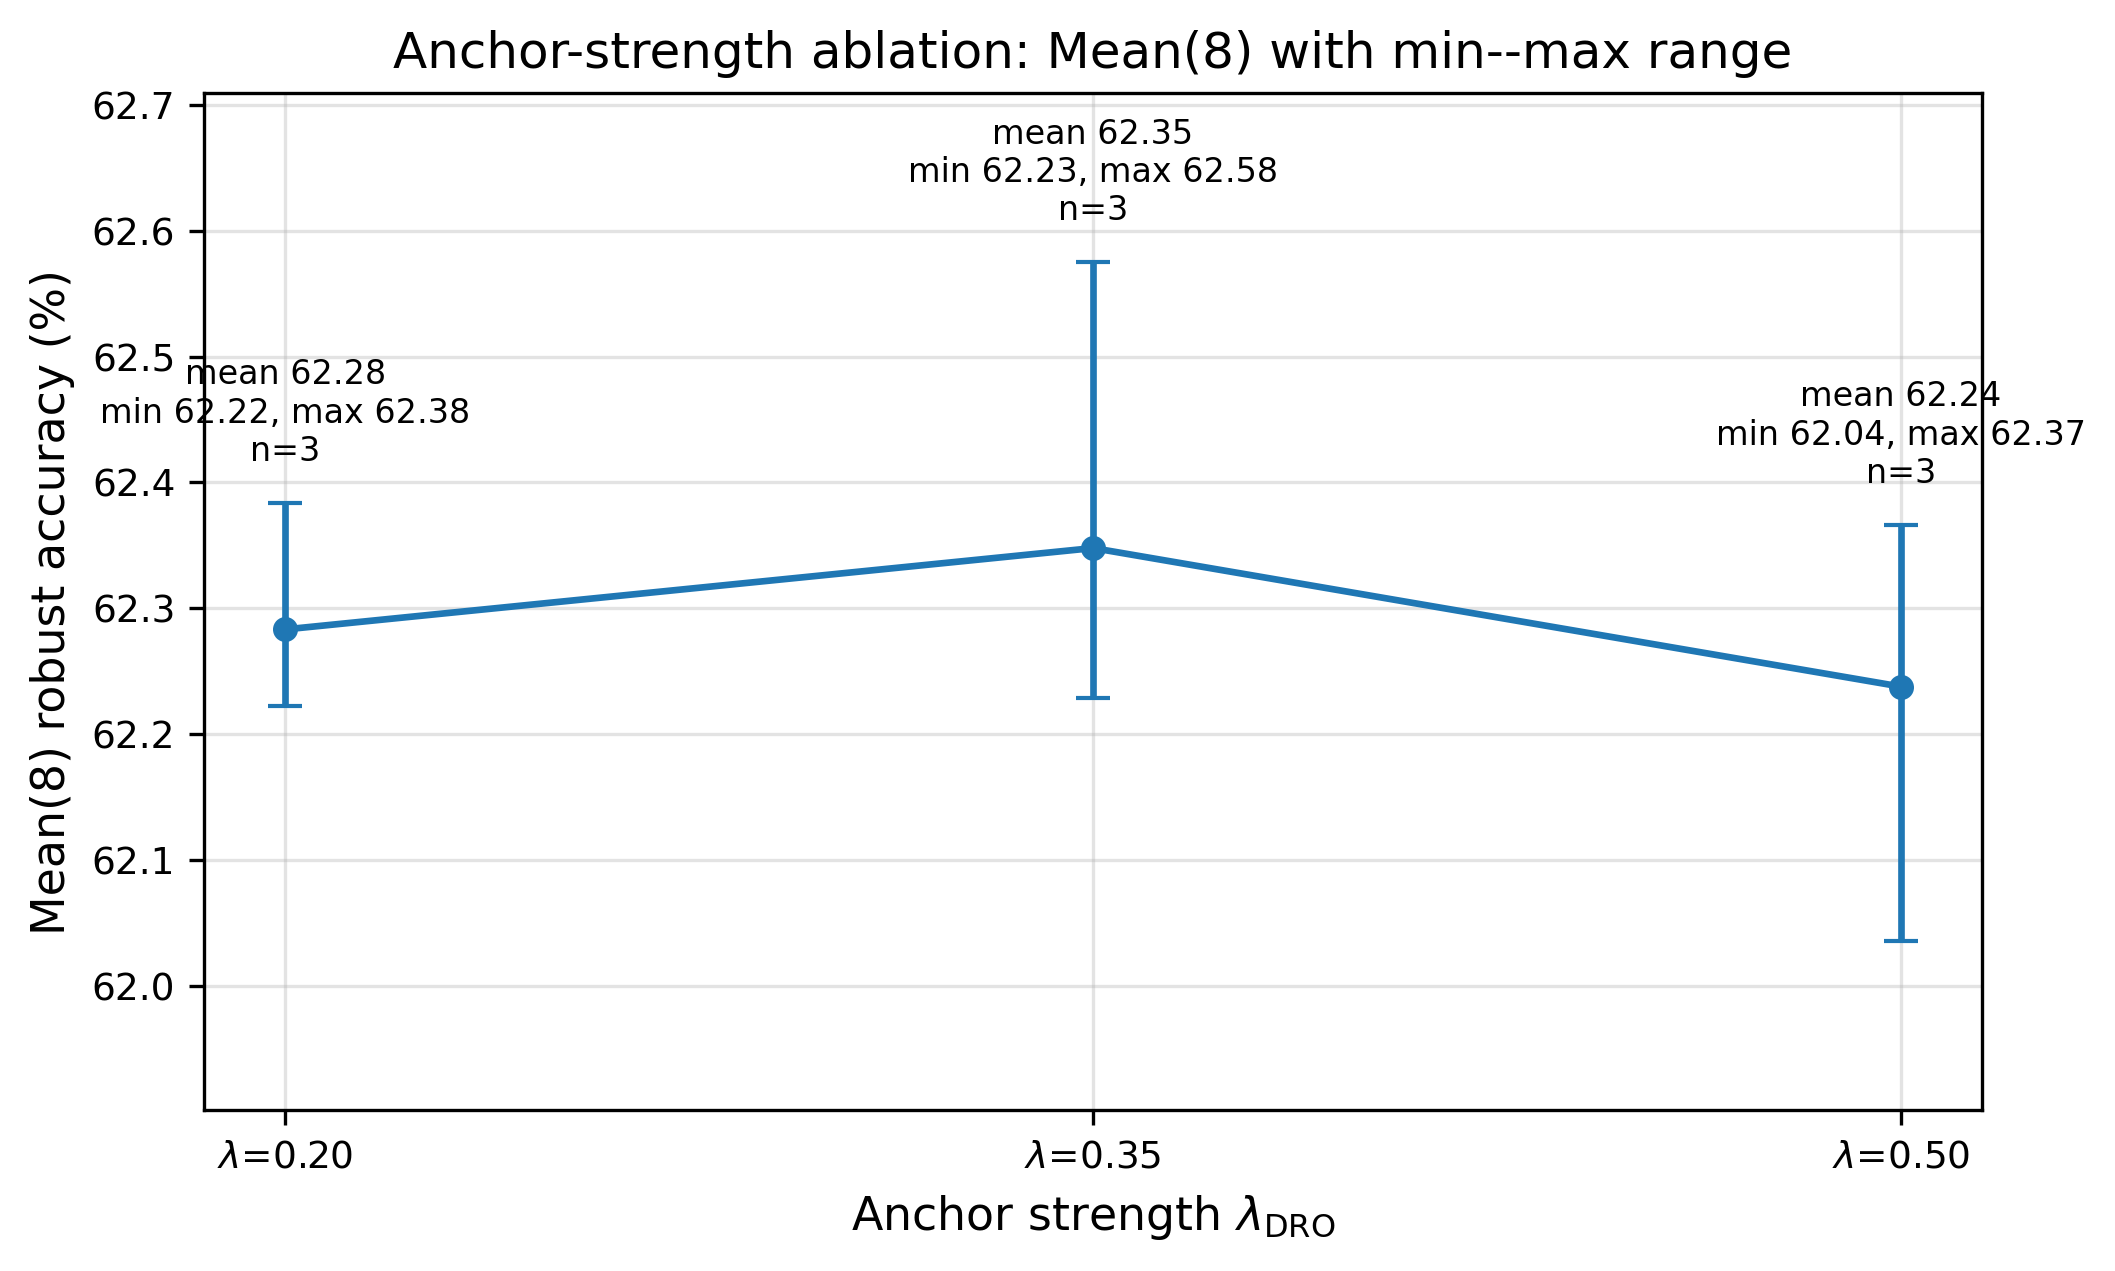
\includegraphics[width=0.82\linewidth]{figures/ablations/ablation_anchor_strength.png}
    \caption{Sensitivity of AttackDRO++ to the anchor strength $\lambda_{\mathrm{DRO}}$. Points show Mean(8) robust accuracy with the min-to-max range across available runs; Mean(8) is computed over the eight non-AutoAttack evaluation attacks. The previous $\lambda_{\mathrm{DRO}}=1.0$ setting is excluded from the final ablation panel.}
    \label{fig:ch6_ablation_anchor_strength}
\end{figure}

Overall, the anchor-strength ablation supports the design motivation from
Chapter~\ref{chap:methodology}. AttackDRO++ benefits from a nonzero
cluster-level correction, but the correction should remain anchored to the
uniform multi-attack objective. The default value
$\lambda_{\mathrm{DRO}}=0.35$ is retained because it gives the best balance
among the tested settings without relying entirely on either uniform ERM or
aggressive Cluster-DRO weighting.

\subsection{Recluster Frequency: How Often Should Groups Update?}
\label{subsec:ch6_ablation_recluster_frequency}

The cluster-refresh interval $R$ controls how often the K-means clusterer is
refitted from the feature bank. Refreshing every epoch may adapt faster to
changes in the representation, but it also changes the group structure more
frequently. Refreshing less often may give a more stable grouping signal, but it
may lag behind the evolving model.

Since the refresh interval trades adaptation speed against group stability,
Table~\ref{tab:ch6_cluster_refresh_schedule_ablation} compares refreshing every
one epoch with refreshing every two epochs. The two schedules produce nearly
identical Mean(8), Worst(8), and family-level behavior. The default two-epoch
schedule gives a slightly higher Mean(8) and $\ell_\infty$-family average, while
the one-epoch schedule gives a slightly higher Worst(8), AutoAttack, and
$\ell_2$-family average. These differences are small relative to the
three-run setting, so the ablation does not show a strong advantage for either
schedule.

\begin{table}[H]
\centering
\caption{Cluster-refresh schedule ablation for AttackDRO++ with
$\lambda_{\mathrm{DRO}}=0.35$, gradient fingerprints, and $K=4$. Values are
robust accuracy (\%) reported as mean $\pm$ standard deviation across three
runs. Mean(8) and Worst(8) are computed over the eight non-AutoAttack attacks;
AutoAttack-$\ell_\infty$ is reported separately. Bold values indicate the best setting for each metric.}
\label{tab:ch6_cluster_refresh_schedule_ablation}
\scriptsize
\setlength{\tabcolsep}{4pt}
\renewcommand{\arraystretch}{1.08}
\resizebox{\textwidth}{!}{%
\begin{tabular}{lcccccc}
\toprule
Refresh interval
& Runs
& Mean(8) $\uparrow$
& Worst(8) $\uparrow$
& AutoAttack $\uparrow$
& $\ell_2$-family avg. $\uparrow$
& $\ell_\infty$-family avg. $\uparrow$ \\
\midrule
1 epoch
& 3
& $62.38 \pm 0.14$
& \bestval{45.17 $\pm$ 0.34}
& \bestval{40.30 $\pm$ 1.37}
& \bestval{67.57 $\pm$ 0.16}
& $57.18 \pm 0.27$ \\

2 epochs (default)
& 3
& \bestval{62.44 $\pm$ 0.22}
& $45.14 \pm 0.23$
& $39.45 \pm 0.68$
& $67.56 \pm 0.08$
& \bestval{57.31 $\pm$ 0.35} \\
\bottomrule
\end{tabular}}
\end{table}

\begin{figure}[H]
    \centering
    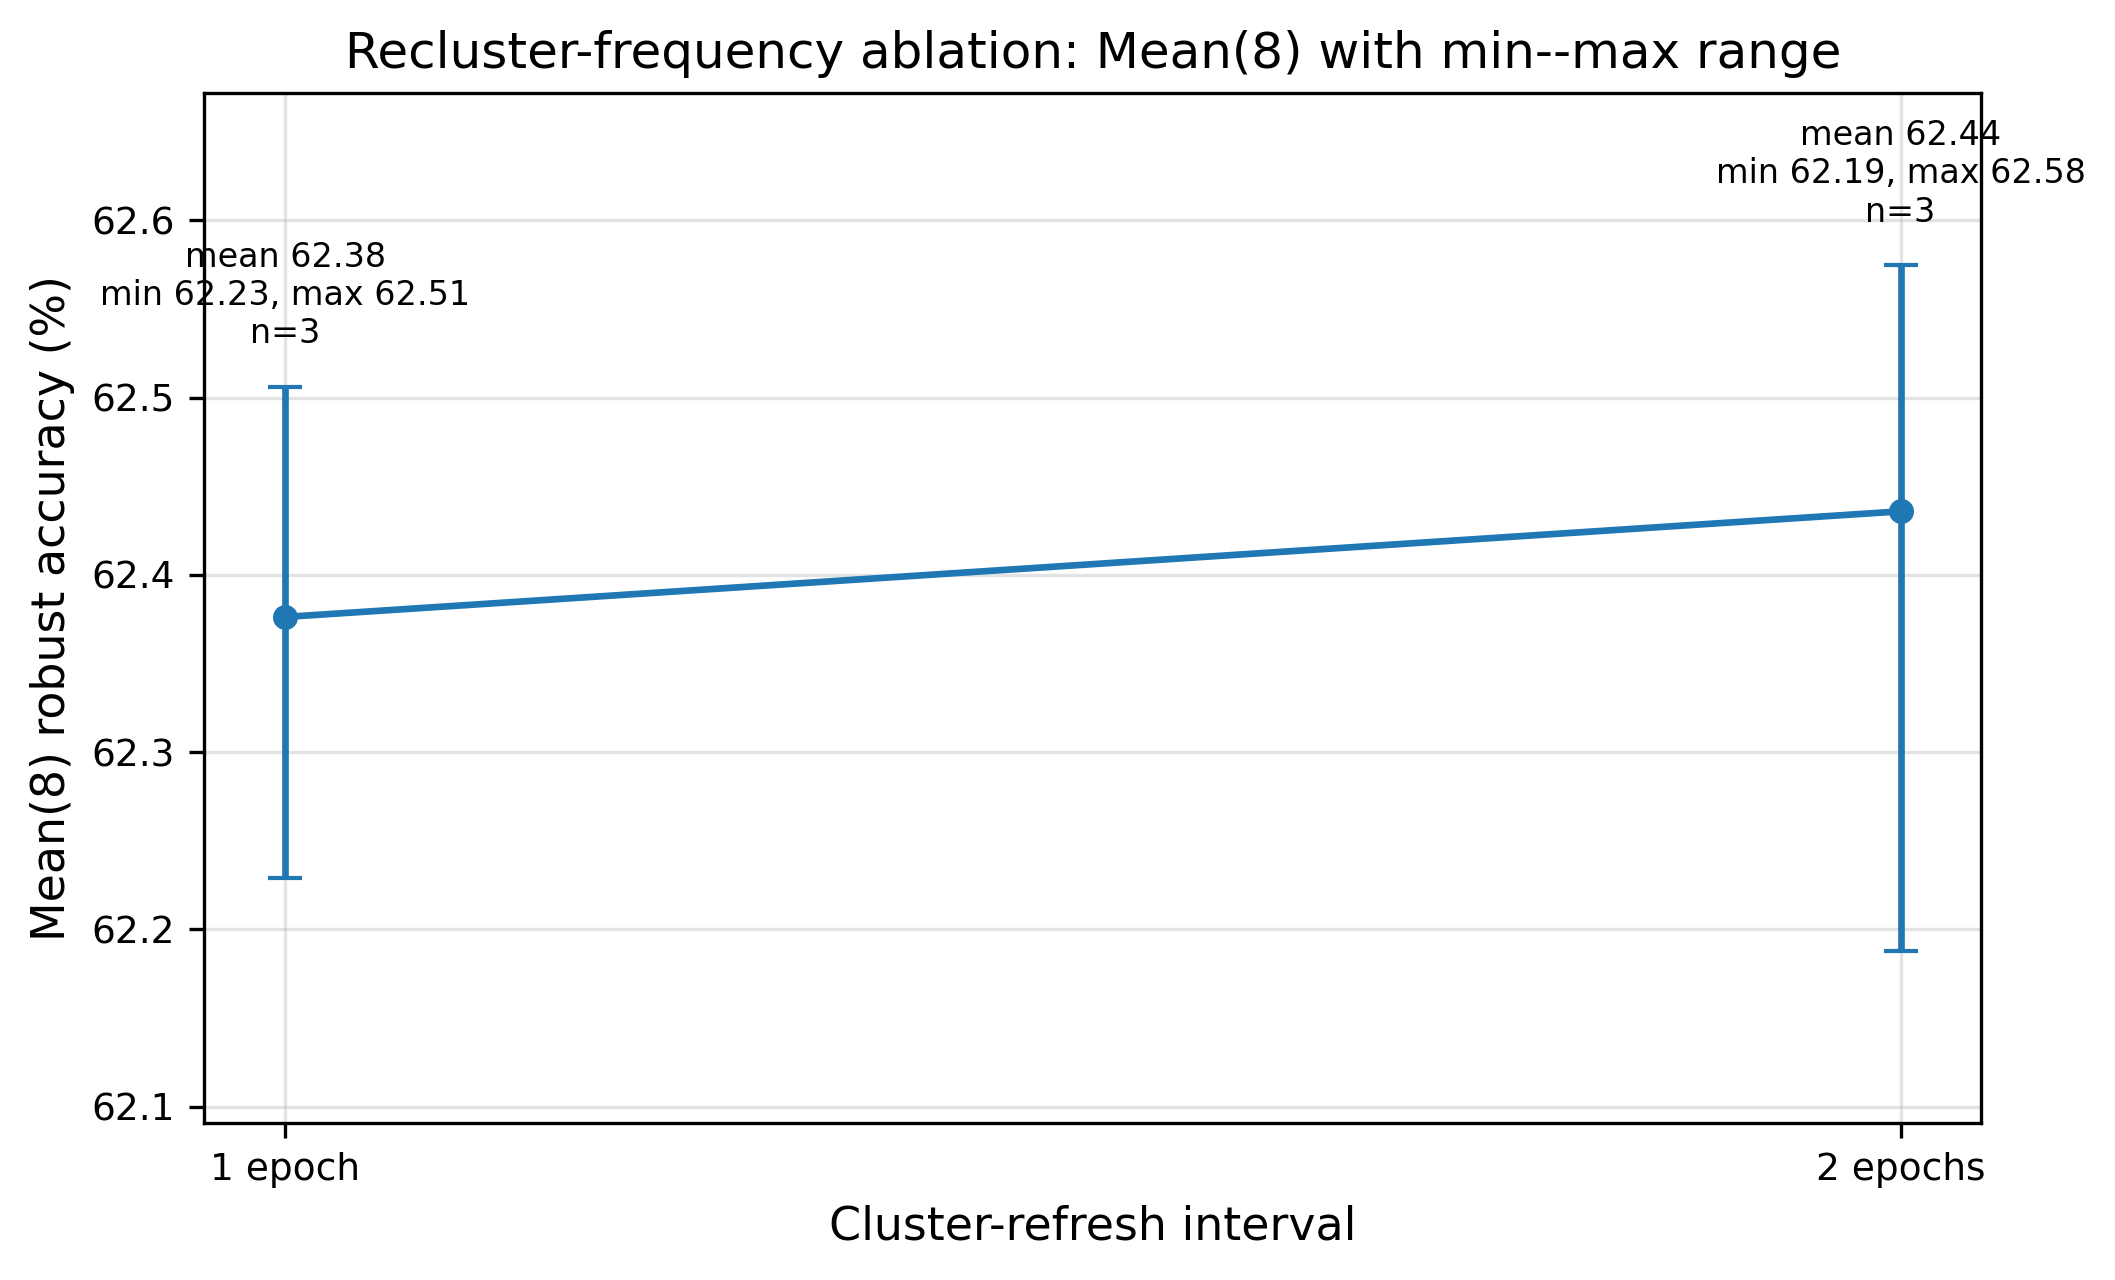
\includegraphics[width=0.82\linewidth]{figures/ablations/ablation_recluster_frequency.png}
    \caption{Sensitivity of AttackDRO++ to the cluster-refresh interval. Points show Mean(8) robust accuracy with the min-to-max range across available runs; Mean(8) is computed over the eight non-AutoAttack evaluation attacks. The two refresh schedules produce similar results, so the default two-epoch schedule is retained as a practical stability choice.}
    \label{fig:ch6_ablation_recluster_frequency}
\end{figure}

We retain $R=2$ epochs as the default because it gives comparable robustness
while reducing the frequency of cluster refitting. This is a practical choice:
the ablation suggests that the method is not highly sensitive to the exact
refresh interval, so the less frequent schedule is preferred for stability and
simplicity.

\paragraph{Supplementary architecture check.}
A single-run WRN-28-10 check is reported in Appendix~\ref{app:extras} as
supplementary evidence. This check is not included in the main paired claims
because it does not use the repeated-random-seed protocol of the main ResNet-18
experiments. In that setting, Multi-AT slightly outperforms AttackDRO++ on both
Mean(8) and AutoAttack-$\ell_\infty$, suggesting that the relative benefit of
the proposed grouping strategy may depend on model capacity and should be
evaluated more systematically in future work.

Together, these ablations suggest that the final AttackDRO++ configuration is
not the result of a fragile hyperparameter choice. Moderate clustering
granularity, moderate anchor strength, and a two-epoch refresh schedule provide a
stable practical configuration. The ablations also define the limits of the
current evidence: they support the selected ResNet-18 configuration, but broader
architecture-level conclusions require additional repeated-seed experiments.
